\documentclass[11pt]{article}
%% Package imports
\usepackage[utf8]{inputenc}
\usepackage{amsmath}
\usepackage{subcaption}
\usepackage{amsfonts}
\usepackage{amssymb}
\usepackage{physics}
\usepackage{graphicx}
\usepackage[left=2cm,right=2cm,top=2cm,bottom=2cm]{geometry}
\usepackage{multirow}
\usepackage{booktabs}
\usepackage{float}
\usepackage{verbatim}
\usepackage{amsthm}
\usepackage{minted}
\usepackage{fancyhdr}
\usepackage{parskip}
\usepackage{minted}
\usepackage[shortlabels]{enumitem}
\renewcommand{\baselinestretch}{1.5}

%% Commands for inserting big braces.
\newcommand\lb{\left\lbrace}
\newcommand\rb{\right\rbrace}

%% Commands for set such that notation
\newcommand\st{\text{ } | \text{ }}

%% Math symbols
\newcommand\Q{\mathbb{Q}}
\newcommand\R{\mathbb{R}}
\newcommand\N{\mathbb{N}}
\newcommand\C{\mathbb{C}}
\newcommand\l{\mathcal{l}}
\newcommand\sucht{\text{ such that }}
\newcommand\weh{\text{ we have }}

\newtheorem*{theorem}{Theorem}
\renewcommand\qedsymbol{$\blacksquare$}

%% Page style settings
\pagestyle{fancy}
\fancyfoot{}
\fancyhead[L]{\slshape{Formalising Mathematics}}
\fancyhead[R]{\slshape{CID: 01871147}}
\fancyfoot[C]{\thepage}
\begin{document}

\title{Formalising Mathematics - Coursework 1 \\ Intermediate Value Theorem}
\date{\today}
\author{CID: 01871147}
\maketitle

\section*{ Introduction }

In the first part of the coursework I've decided to formalise the intermediate
value theorem which was covered as a part of the course MATH40002: Analysis I
during the first year of my degree. My choice of this theorem was motivated by
the fact that the next two parts of the coursework need to cover concepts that
I've learned in my second and third year of the course respectively. Because of
this, and the fact that as a JMC student I only took one other maths module this
term (which is MATH60029: Functional Analysis), I needed to start building up my
knowledge of formalising proofs in mathematical analysis.

This report documents the process of formalising IVT using the Lean programming
language. It is a functional language which can also be used as an interactive
theorem prover. Programming in Lean involves using a wide range of tools, which
given a set of hypotheses allow the programmer to prove a certain statement
(later referred to as the goal). Those tools are called "tactics" in Lean.
These tactics allow the user to perform usual manipulations on the state of the
argument (e.g. introduction of hypotheses).

The main advantage of using Lean in order to formalise a theorem is that we can
easily modularise the argument into a set of lemmas which we can then combine
in order to get our desired proof. This is achieved because Lean is a
functional programming language and so the proofs that we formulate are
actually represented as functions which take hypotheses as input and return the
proof of a particular claim a output. That way formulating a proof can in some
cases be thought of as a function composition.

\pagebreak

\section*{ Proof of IVT }

Before we go over the process of formalising the theorem, let us start by
considering the proof of it which I followed when formalising the theorem.
\begin{theorem}[Intermediate Value Theorem]
  Let $f : [a, b] \to \R  $ be a continuous function, then for all $c$ between
  $f(a)$ and $f(b)$, there exists $x \in [a, b] $ satisfying $f(x) = c$.
\end{theorem}

\begin{proof}
  Let us first assume without loss of generality that $f(a) < c < f(b)$. We can
  do this because if we consider the other possible cases, we get the following:
  \begin{itemize}
    \item if either $f(a) = c$ or $f(b) = c$ we take $a$ or $b$ respectively
      and the claim follows;
    \item if $f(a) = f(b)$ then c = f(a) and we are done;
    \item if instead $f(a) < f(b)$, we define $g(x) = -f(x)$, and thus
      $g(a) < g(b)$. Now we are back in the first case with $g(a) < -c < g(b)$,
      and so we need to find an $x$ such that $g(x) = - c$ which in turn implies
      that $f(x) = c$ and we are done.
  \end{itemize}

Note that the case analysis above will be important in the formal proof in
Lean. It allowed me to prove the theorem just for the case $f(a) < c < f(b)$ as
a separate lemma and then reuse it in the main body of the proof.

Now we can define the following set:
\[
  S = \lbrace y \in [a, b] | f(y) < c\rbrace
.\]

We'll show that it has a supremum $x$ and that it satisfies $f(x) = c$. First,
observe that $S$ is nonempty, as $ a \in S $, and it is also bounded above by
$b$. Therefore, we may deduce that $S$ has a supremum and also if we let
$x = \sup S$, it satisfies $a \le x \le b$.

In what follows, we'll show that $f(x) \ge c$ and  $f(x) \le c$ and so our goal
will follow from antisymmetry.

To show that $f(x) \ge c$ let us argue by contradiction and assume $f(x) < c$.
In in this case, we'll use continuity at  $x$ with  $\epsilon = c - f(x) $
which satisfies  $\epsilon > 0$. Observe that now if $f(x) < c$ then as $c <
f(b)$, we deduce  $x \ne b$, thus we get  $x < b$. Using continuity at x, we have:
\[
\exists \delta > 0 \sucht \forall y \in [a, b] \weh | x - y | < \delta \implies |f(y) - f(x)| < \epsilon .\]

By considering the second case in the expression $|f(y) - f(x)| < \epsilon $ above
we can deduce that:
\[
  \forall y \in (x - \delta, x + \delta) \cap [a, b] \weh f(y) < f(x) + \epsilon = c
.\]

Therefore, we can deduce that  all $y$ above belong to $S$.
If we now choose e.g. $y = x + \frac{1}{2} \min(\delta, b - x)$. We have found
a $y$ which is greater than $x$ and belongs to $S$. However,  $x$ was supposed
to be an upper bound for  $S$, so we have a contradiction.

For the second case $f(x) \le c$, we again argue by contradiction. Similarly to
the previous reasoning, we assume that $f(x) > c$ and deduce that  $x \ne a$.
We let  $\epsilon = f(x) - c > 0$ and by continuity of $f$ at $x$, we obtain a
$\delta > 0$ such that:
\begin{equation}
  \forall y \in (x - \delta, x + \delta) \cap [a, b] \weh |f(y) - f(x)| < \epsilon
.\end{equation}

Now, similar as before, if for some $y$ we have  $|f(y) - f(x)| < \epsilon$, then
in particular $f(x) - \epsilon < f(y) $ and by our definition of  $\epsilon$,
we have $f(x) - \epsilon = c $. We get  $c < f(y)$, and none of such
$y$ belong to $S$. By letting:
\[
m = \max \left(x - \frac{\delta}{2}, a\right)
,\]
we can observe that $m < x$ and moreover $(m, x) \subset (x - \delta, x + \delta) \cap [a, b]$
So if we apply the property $(1)$ above, we may deduce that for all $y \in (m, x)$
we have  $y \not\in S$. Therefore, $m$ is an upper bound for $S$, however it is
less than $x$, which contradicts with  $x$ being the least upper bound.

Hence we deduce that both $f(x) \ge c$ and  $f(x) \le c$ are satisfied, thus,
by antisymmetry, we have $f(x) = c$ which we had to show.
\end{proof}

In the next sections I will explain the methodology that I used to
formalise the theorem, and contrast the proof above with the implementation
that I developed in Lean to formalise it.
\section*{ The Process of Formalising }
In order to formalise the theorem I took the following approach. First, I
started by formulating a hand-written proof of the theorem using the course
notes. After I familiarised myself with the argument, I tried to directly
translate it into the Lean code without thinking about the overall structure of
the argument.

The interactive theorem proving in Lean works similarly to compiling a program
in any given programming language. The programmer is writing the code in the
editor, while simultaneously the Lean language server protocol is trying to
"compile" the code which effectively checks the validity of the proof (and
incomplete or incorrect proof results in a compilation error). Consequently, if
the proof that we write is correct, then Lean should compile it without
producing any errors.

After trying to formalise my argument in one monolithic proof, I eventually
managed to complete it and successfully compile. The main issue I
encountered was that because of the lack of modularity, the proof was very long
and the compilation times were about 5-6 seconds. At some point it started
negatively affecting my experience of using the language, as I couldn't quickly
make adjustments to the proof and see the instant response from the compiler.

\begin{figure}[H]
  \centering
  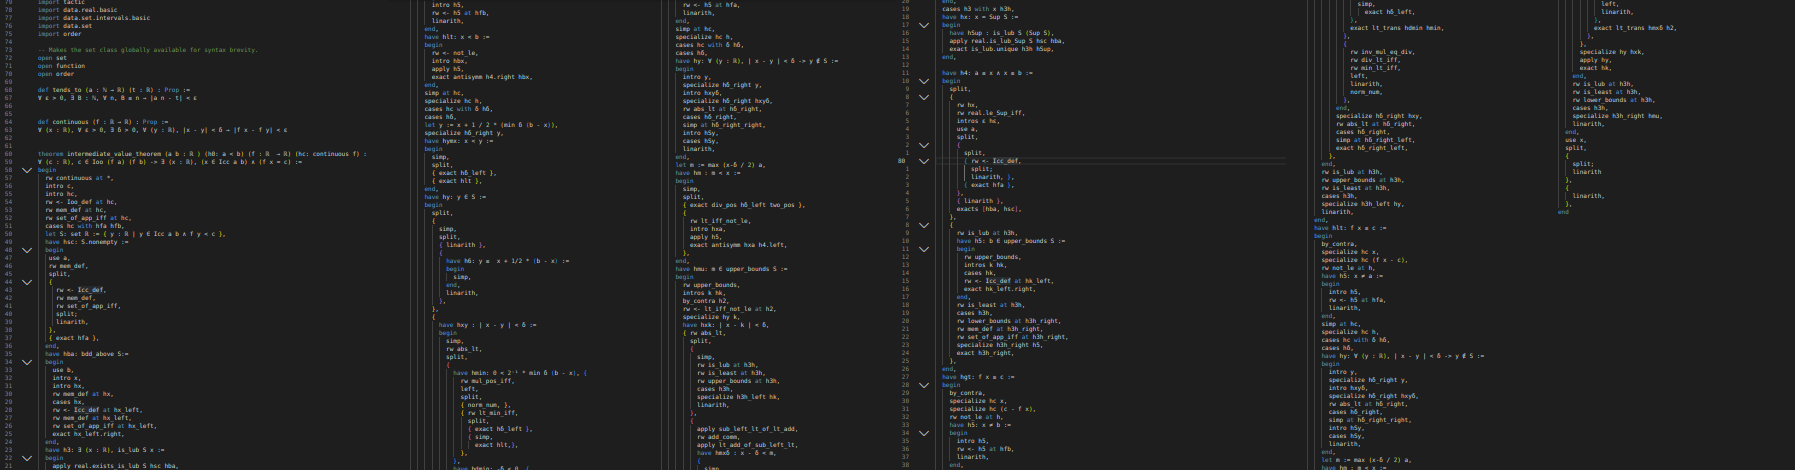
\includegraphics[scale=1.1]{long_code.png}
  \caption{The first inefficient version of the proof}
	\label{long_code}

\end{figure}

In order to solve this issue, I've decided to introduce multiple lemmas, which
aimed at proving facts which are true in general settings and were used within
my argument. I also isolated the special case of the theorem which was then
used to prove the main statement in full generality.

This change of approach allowed me to get a better understanding of the actual
proof, I needed to identify the parts of it which were true in a more general
setting and abstract them out into their separate lemmas.

\begin{minted}{lean}
 def continuous (f : ℝ → ℝ) : Prop :=
∀ (x : ℝ), ∀ ε > 0, ∃ δ > 0, ∀ (y : ℝ), |x - y| < δ → |f x - f y| < ε

\end{minted}

\section*{ Conclusion }

\end{document}














